\documentclass[a4paper,10pt]{article}
\usepackage[utf8x]{inputenc}
\usepackage[utf8x]{inputenc}
\usepackage[OT1]{fontenc}
\usepackage{hyperref}
\usepackage{Sweave}
\usepackage{graphicx}
\usepackage{color}
\graphicspath{figures/}
\usepackage{float}
\usepackage{wrapfig}
\usepackage{subfigure}
%% Package to linebreak URLs in a sane manner.
\usepackage{url}
%% Define a new 'smallurl' style for the package that will use a smaller font.
\makeatletter
\def\url@smallurlstyle{%
  \@ifundefined{selectfont}{\def\UrlFont{\sf}}{\def\UrlFont{\small\ttfamily}}}
\makeatother
%% Now actually use the newly defined style.
\urlstyle{smallurl}
%% Define 'tinyurl' style for even smaller URLs (such as in tables)
\makeatletter
\def\url@tinyurlstyle{%
  \@ifundefined{selectfont}{\def\UrlFont{\sf}}{\def\UrlFont{\scriptsize\ttfamily}}}
\makeatother
%% Make margins less ridiculous
\usepackage{fullpage}
%% Make URLs clickable
%\usepackage[colorlinks, bookmarks=false]{hyperref}
%\usepackage[colorlinks, bookmarks=true]{hyperref}
%% Since I'm using the LaTeX Makefile that uses dvips, I need this
%% package to make URLs break nicely
\usepackage{breakurl}
\usepackage{todonotes}
\usepackage{amsmath,amsfonts}
\numberwithin{equation}{subsection}
%%\usepackage{nonfloat}
\usepackage{bbm}
\usepackage{setspace}
\onehalfspacing
\usepackage{tabularx}

%
%
%
\usepackage{listings}
\usepackage{courier}
\lstset{
         basicstyle=\footnotesize\ttfamily, % Standardschrift
         %numbers=left,               % Ort der Zeilennummern
         numberstyle=\tiny,          % Stil der Zeilennummern
         stepnumber=2,               % Abstand zwischen den Zeilennummern
         numbersep=5pt,              % Abstand der Nummern zum Text
         tabsize=2,                  % Groesse von Tabs
         extendedchars=true,         %
         breaklines=true,            % Zeilen werden Umgebrochen
         keywordstyle=\color{red},
    		frame=b,         
 %        keywordstyle=[1]\textbf,    % Stil der Keywords
 %        keywordstyle=[2]\textbf,    %
 %        keywordstyle=[3]\textbf,    %
 %        keywordstyle=[4]\textbf,   \sqrt{\sqrt{}} %
         stringstyle=\color{white}\ttfamily, % Farbe der String
         showspaces=false,           % Leerzeichen anzeigen ?
         showtabs=false,             % Tabs anzeigen ?
         xleftmargin=17pt,
         framexleftmargin=18pt,
         framexrightmargin=6pt,
         framexbottommargin=4pt,
         %backgroundcolor=\color{lightgray},
         showstringspaces=false      % Leerzeichen in Strings anzeigen ?        
 }
 \lstloadlanguages{% Check Dokumentation for further languages ...
         %[Visual]Basic
         %Pascal
         %C
         %C++
         %XML
         %HTML
         %Java
 }
%\DeclareCaptionFont{blue}{\color{blue}} 
%\captionsetup[lstlisting]{singlelinecheck=false, labelfont={blue}, textfont={blue}}
\usepackage{caption}
\DeclareCaptionFont{white}{\color{white}}
\DeclareCaptionFormat{listing}{\colorbox[cmyk]{0.43, 0.35, 0.35,0.01}{\parbox{\textwidth}{\hspace{15pt}#1#2#3}}}
\captionsetup[lstlisting]{format=listing,labelfont=white,textfont=white, singlelinecheck=false, margin=0pt, font={bf,footnotesize}}
%
%

%opening
\title{Sanity check and the Trajectory workflow test}
\author{Pavel Senin}

\begin{document}

\maketitle

\begin{abstract}
This document is a workflow primer.
\end{abstract}

\section{Aggregating commits statistics in TrajectoryDB}
For the first test I have selected a contributor with id \emph{153} and a project with id \emph{18} (android-kernel-omap). 
As a daytime interval I have chosen the \emph{NT} interval corresponding to night hours from \emph{5PM to 00AM}. 
Let's the see records in the change database first by querying it with the query from listing \ref{query1}:
\begin{lstlisting}[label=query1,caption=Data summary retrieval SQL query]
select c.id, c.author_date, c.subject, sum(c.added_files) ta, 
 sum(c.edited_files) te, sum(c.removed_files) td, sum(c.added_lines) la, 
 sum(c.edited_lines) le, sum(c.removed_lines) ld from android_change c 
 where c.author_id=153 and c.project_id=18 
 AND c.author_date between "2010-03-01" AND "2010-04-01"
 and date_format(c.author_date,'%H') between 17 and 23
 group by c.id order by c.author_date;
\end{lstlisting}

The DB output is shown in Table \ref{tab:first}.

\begin{table}[h]
  \tiny
  \label{tab:first}
  \caption{Result of running the query \ref{query1} against the TrajectoryDB. }
  \begin{tabularx}{\textwidth}{ | l | l | X | r | r | r | r | r | r | r |}
  \hline           
id & author\_date & subj & ta & te & td & la & le & ld\\ 
\hline           
827962 & 2010-03-03 17:08 & \verb7sparc64: Kill off old sys_perfctr system call and state.7 & 0 & 12 & 0 & 0 & 18 & 195\\ 
827955 & 2010-03-03 18:06 & \verb1sparc64: Make prom entry spinlock NMI safe.1 & 0 & 1 & 0 & 0 & 7 & 0\\ 
827241 & 2010-03-05 22:41 & \verb1timbgpio: fix build1 & 0 & 1 & 0 & 1 & 0 & 0\\ 
826446 & 2010-03-10 22:05 & \verb1uartlite: Fix build on sparc.1 & 0 & 1 & 0 & 0 & 5 & 0\\ 
825982 & 2010-03-13 21:17 & \verb1Merge branch 'master' of1 & 0 & 0 & 0 & 0 & 0 & 0\\
& & \verb1git://git.kernel.org/pub/scm/linux/kernel/git/linville/wireless-2.61 &  &  &  &  &  & \\  
825784 & 2010-03-15 23:23 & \verb7e100: Fix ring parameter change handling regression.7 & 0 & 1 & 0 & 0 & 1 & 0\\ 
825679 & 2010-03-16 22:37 & \verb1bridge: Make first arg to deliver_clone const.1 & 0 & 1 & 0 & 0 & 4 & 0\\ 
825678 & 2010-03-16 22:40 & \verb7sunxvr1000: Add missing FB=y depenency.7 & 0 & 1 & 0 & 0 & 1 & 0\\ 
825288 & 2010-03-20 22:41 & \verb1Merge branch 'vhost' of 1 & 0 & 0 & 0 & 0 & 0 & 0\\
& & \verb1git://git.kernel.org/pub/scm/linux/kernel/git/mst/vhost1 &  &  &  &  &  & \\  
825287 & 2010-03-20 23:24 & \verb1Merge branch 'master' of 1 & 0 & 0 & 0 & 0 & 0 & 0\\ 
& & \verb1master.kernel.org:/pub/scm/linux/kernel/git/davem/net-2.61 &  &  &  &  &  & \\  
824847 & 2010-03-25 19:48 & \verb1Merge branch 'master' of 1 & 0 & 0 & 0 & 0 & 0 & 0\\ 
& & \verb1git://git.kernel.org/pub/scm/linux/kernel/git/kaber/nf-2.61 &  &  &  &  &  & \\  
824789 & 2010-03-26 18:23 & \verb7Revert r8169: enable 64-bit DMA by default for PCI Express devices (v2)"7 & 0 & 1 & 0 & 4 & 3 & 8\\ 
824627 & 2010-03-29 22:08 & \verb1sparc64: Properly truncate pt_regs framepointer in perf callback.1 & 0 & 1 & 0 & 0 & 1 & 0\\ 
824620 & 2010-03-29 22:50 & \verb1Merge branch 'master' of 1 & 0 & 0 & 0 & 0 & 0 & 0\\
& & \verb1git://git.kernel.org/pub/scm/linux/kernel/git/linville/wireless-next-2.61 &  &  &  &  &  & \\  
\hline           
  \end{tabularx}
\end{table}
 Five of 14 commits: \emph{825982, 825288, 825287, 824847, 824620} are merge commits. 
I am unable to collect any of the statistics about these, which is the first question I am saving for future: 
\textit{should I count these merege commits (which have zero statistics) as an activity or should I skip commits which have
zero changes attached?} I think I should include these into analyses since even if the change appears to be empty
it takes some time and effort to actually make a merge decision, to perform the merge, and to check the merge results.

I have checked the recall of that change by Trajectory, see Figure \ref{fig:git_screen}, it seems to be that Git doesn't have any 
data about the merge, maybe it can be recalled by traversing the tree up or down, but this is not implemented.

\begin{wrapfigure}{lh}{1.0\textwidth}
   \begin{center}
   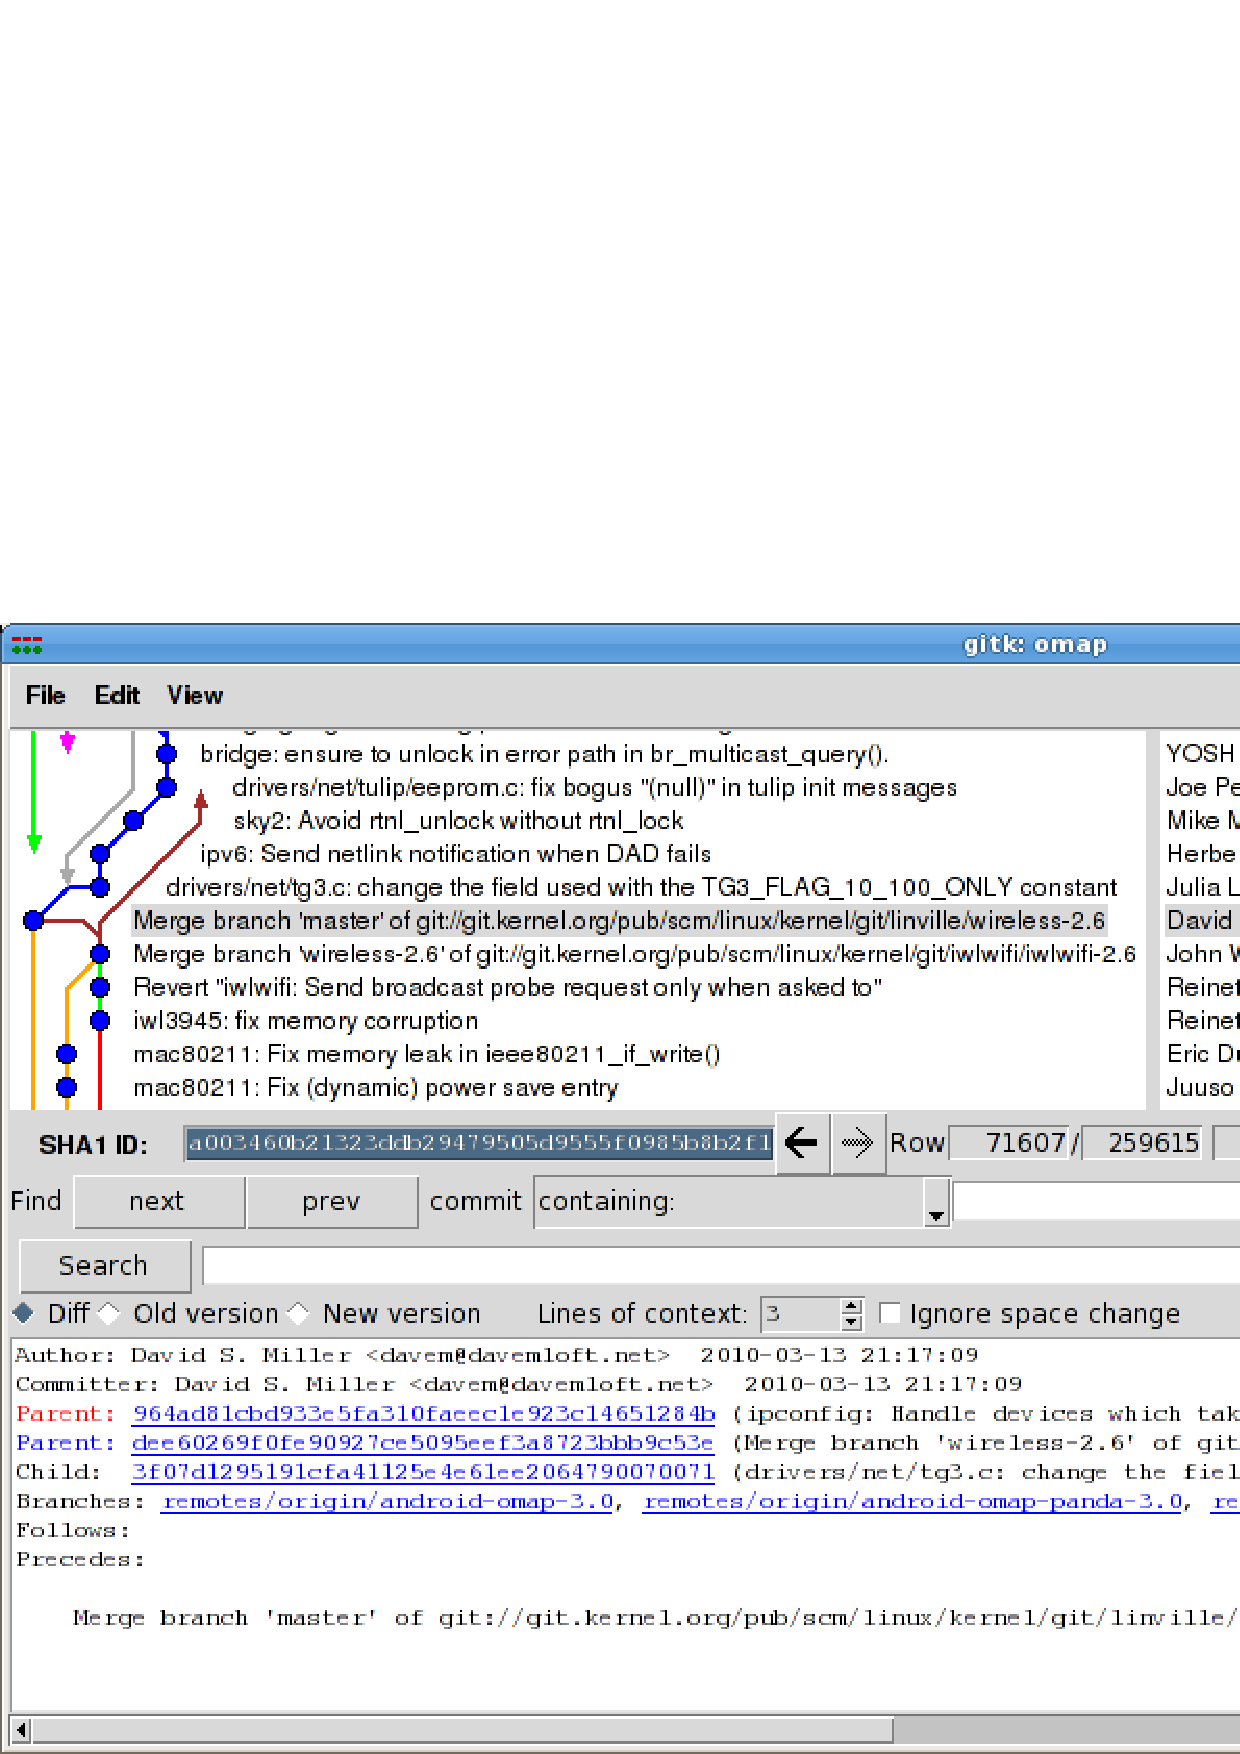
\includegraphics[scale=1.0,width=1.0\textwidth]{figures/Screenshot-gitk:omap.png}
   \end{center}
   \caption{The GUI git viewer screenshoot illustrating commit statistics.}
   \label{fig:git_screen}
\end{wrapfigure}

\clearpage
However, the result shown in Table \ref{tab:first} is not very suitable for further analyses because changes are 
not aggregated by date, let's fix this by running the query from liting \ref{query2} which I in fact use within the 
Trajectory workflow.
\begin{lstlisting}[label=query2,caption=Data summary retrieval SQL query with aggergation by date]
select date_format(c.author_date, '%Y-%m-%d') as day, count(distinct(c.id)) as commits, 
 sum(c.added_files) as added_files, sum(c.edited_files) as edited_files, sum(c.removed_files) as removed_files, 
 sum(c.added_lines) as added_lines, sum(c.edited_lines) as edited_lines, sum(c.removed_lines) as removed_lines 
 FROM android_change c 
 where c.author_id=153 and c.project_id=18 
 and c.author_date between "2010-03-01" AND "2010-04-01"
 and date_format(c.author_date,'%H') between 17 and 23 
 group by date_format(c.author_date, '%Y%m%d');
\end{lstlisting}

\begin{table}[h]
  \label{tab:second}
  \caption{Result of running the query \ref{query2} against the TrajectoryDB.}
  \begin{tabularx}{400pt}{ | X | r | r | r | r | r | r | r | }
  \hline           
day & commits & added\_fs & edited\_fs & rm\_fs & added\_ls & edited\_ls & rm\_ls\\ 
\hline           
2010-03-03 & 2 & 0 & 13 & 0 & 0 & 25 & 195\\ 
2010-03-05 & 1 & 0 & 1 & 0 & 1 & 0 & 0\\ 
2010-03-10 & 1 & 0 & 1 & 0 & 0 & 5 & 0\\ 
2010-03-13 & 1 & 0 & 0 & 0 & 0 & 0 & 0\\ 
2010-03-15 & 1 & 0 & 1 & 0 & 0 & 1 & 0\\ 
2010-03-16 & 2 & 0 & 2 & 0 & 0 & 5 & 0\\ 
2010-03-20 & 2 & 0 & 0 & 0 & 0 & 0 & 0\\ 
2010-03-25 & 1 & 0 & 0 & 0 & 0 & 0 & 0\\ 
2010-03-26 & 1 & 0 & 1 & 0 & 4 & 3 & 8\\ 
2010-03-29 & 2 & 0 & 1 & 0 & 0 & 1 & 0\\
\hline    
  \end{tabularx}
\end{table}
This looks much better - for every day I have aggregated data about number commits, added, edited, deleted files (\emph{added\_fs, edited\_fs, rm\_fs}),
and lines (\emph{added\_ls, edited\_ls, rm\_ls}).
\clearpage

These I save into the separate table (\emph{time\_patterns}) which keeps aggregated data along with the daytime tag. 
I use \emph{NT} tag for the night commits. Let's check the table by running the query from query \ref{query3}:

\begin{lstlisting}[label=query3,caption=Data summary from time\_patterns table]
SELECT * FROM time_patterns WHERE project_id = 18
AND author_id=148 AND UPPER(dtag)=UPPER("NT")
AND day between "2010-03-01" AND "2010-04-01"
ORDER BY day ASC;
\end{lstlisting}

The reason to keep all the data separate is to save the computation time. Running aggregation by time slot and summarizing changes 
as in query \ref{query2} could take a very long time over large repositories, whether running single \emph{SELECT} over 
indexed by user, project, dtag and day \emph{time\_patterns} table takes fraction of a second.


\begin{table}[h]
  \label{tab:third}
  \caption{Result of running the query \ref{query3} against the TrajectoryDB.}
  \begin{tabularx}{400pt}{ | X | r | r | r | r | r | r | r | r |}
  \hline           
day & dtag & commits & t\_ad & t\_ed & t\_dlt & l\_ad & l\_ed & l\_dlt\\ 
\hline           
2010-03-03 & nt & 2 & 0 & 13 & 0 & 0 & 25 & 195\\ 
2010-03-05 & nt & 1 & 0 & 1 & 0 & 1 & 0 & 0\\ 
2010-03-10 & nt & 1 & 0 & 1 & 0 & 0 & 5 & 0\\ 
2010-03-13 & nt & 1 & 0 & 0 & 0 & 0 & 0 & 0\\ 
2010-03-15 & nt & 1 & 0 & 1 & 0 & 0 & 1 & 0\\ 
2010-03-16 & nt & 2 & 0 & 2 & 0 & 0 & 5 & 0\\ 
2010-03-20 & nt & 2 & 0 & 0 & 0 & 0 & 0 & 0\\ 
2010-03-25 & nt & 1 & 0 & 0 & 0 & 0 & 0 & 0\\ 
2010-03-26 & nt & 1 & 0 & 1 & 0 & 4 & 3 & 8\\ 
2010-03-29 & nt & 2 & 0 & 1 & 0 & 0 & 1 & 0\\
\hline    
  \end{tabularx}
\end{table}
\clearpage

\section{Indexing aggregated commits statistics with SAX}
For the data similar to one from table \ref{tab:third} I



\section{Note to myself: wrong counts}
\begin{lstlisting}[label=query_wrong,caption=Wrong counts here at second query due to the join. Look at the results of the third query to understand why]
select date_format(c.author_date, '%Y-%m-%d') as day, count(distinct(c.id)) as commits, 
sum(c.added_files) as added_files, sum(c.edited_files) as edited_files, 
sum(c.removed_files) as removed_files, sum(c.added_lines) as added_lines, 
sum(c.edited_lines) as edited_lines, sum(c.removed_lines) as removed_lines 
FROM android_change c 
where c.author_id=153 and c.project_id=18 
and c.author_date between "2010-03-01" AND "2010-04-01"
 and date_format(c.author_date,'%H') between 17 and 23 
group by date_format(c.author_date, '%Y%m%d');

select date_format(c.author_date, '%Y-%m-%d') as day, count(distinct(c.id)) as commits, 
count(t.change_id) as t, sum(c.added_files) as added_files, sum(c.edited_files) 
as edited_files, sum(c.removed_files) as removed_files, sum(c.added_lines) as added_lines, 
sum(c.edited_lines) as edited_lines, sum(c.removed_lines) as removed_lines 
FROM android_change c 
left join change_target t on c.id=t.change_id
where c.author_id=153 and c.project_id=18 
and c.author_date between "2010-03-01" AND "2010-04-01"
 and date_format(c.author_date,'%H') between 17 and 23 
group by date_format(c.author_date, '%Y%m%d');

select c.*, t.*
FROM android_change c 
left join change_target t on c.id=t.change_id
where c.author_id=153 and c.project_id=18 
and c.author_date between "2010-03-01" AND "2010-04-01"
 and date_format(c.author_date,'%H') between 17 and 23;
\end{lstlisting}

\end{document}
